\documentclass{beamer}

\usepackage[T1]{fontenc}
\usepackage[utf8]{inputenc}
\usepackage[english]{babel}
\usepackage{lmodern}

% Use Unipd as theme, with options:
% - pageofpages: define the separation symbol of the footer page of pages (e.g.: of, di, /, default: of)
% - logo: position another logo near the Unipd logo in the title page (e.g. department logo), passing the second logo path as option 
% Use the environment lastframe to add the endframe text
\usetheme[pageofpages=of]{Unipd}

\title{ \textbf{ \textit{SMKIT} } }
\subtitle{ \textbf{ \textit{Design and development of a social media kit} } }
\author[ \textbf{ \textit{Abdelilah Lahmer} } ]{ \textbf{ \textit{Lahmer Abdelilah} } }

\date{ \textbf{ \textit{December 12, 2024} } }

% The next block of commands puts the table of contents at the beginning of each section and highlights the current section
\AtBeginSection[]
{
  \begin{frame}
    \frametitle{Table of Contents}
    \tableofcontents[currentsection]
  \end{frame}
}



\begin{document}

% Make the title page
\frame{\titlepage}

% Insert the general toc
\begin{frame}{Table of Contents}
    \tableofcontents    
\end{frame}


\section{Introduction}
    \begin{frame}{Introduction to SMKIT}
        \vspace{0.5cm}
        \begin{itemize}
            \item \textbf{SMKIT} stands for \textbf{Social Media KIT}.
            \item A modular tool for automating social media and web content posting.
            \item Designed to process web and local pages, extract metadata, and generate posts for various social platforms.
        \end{itemize}

        \begin{center}
            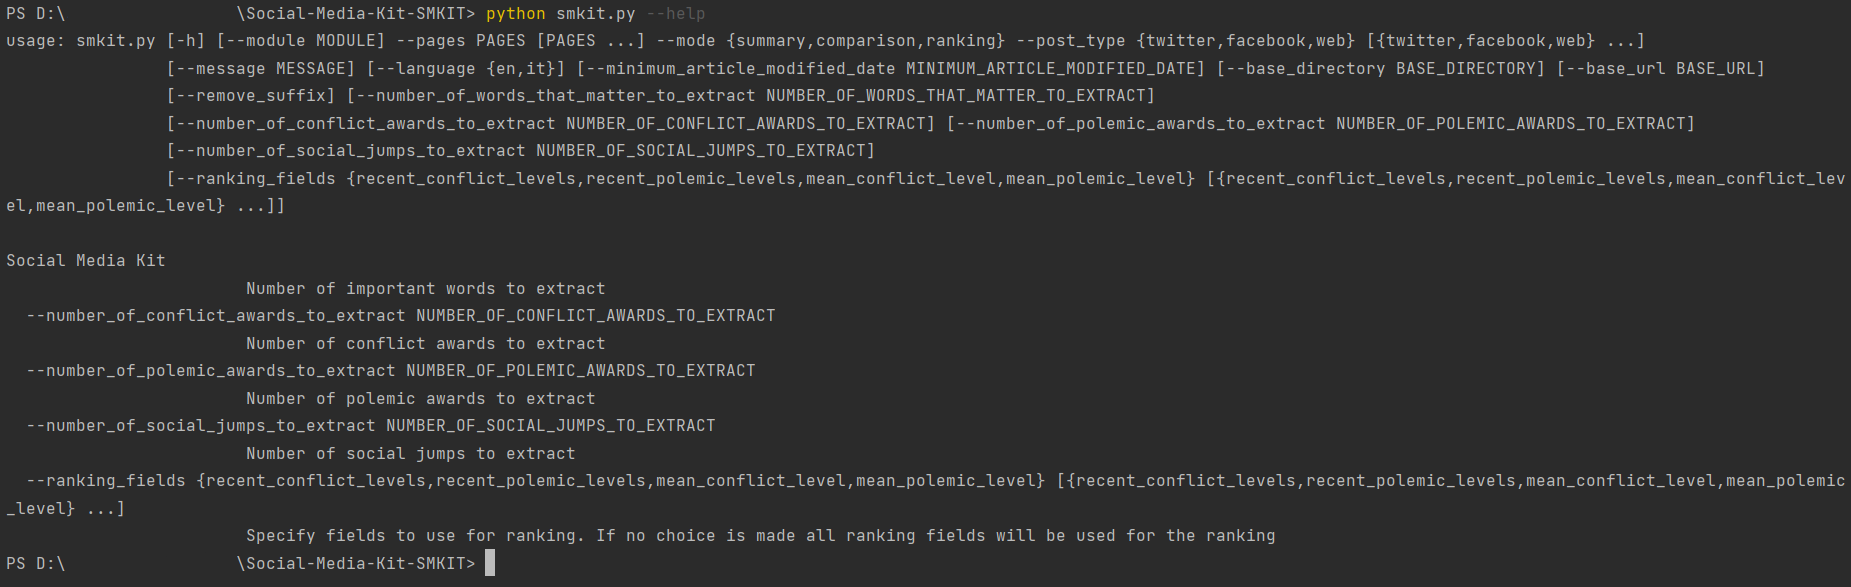
\includegraphics[width=\textwidth, keepaspectratio]{images/introduction_and_motivation_introduction_to_smkit_slide_image.png}
        \end{center}
    \end{frame}

    \begin{frame}{Background}
        \begin{columns}[T]
            \column{0.25\textwidth}
            \vspace{-0.25cm}
            \begin{center}
                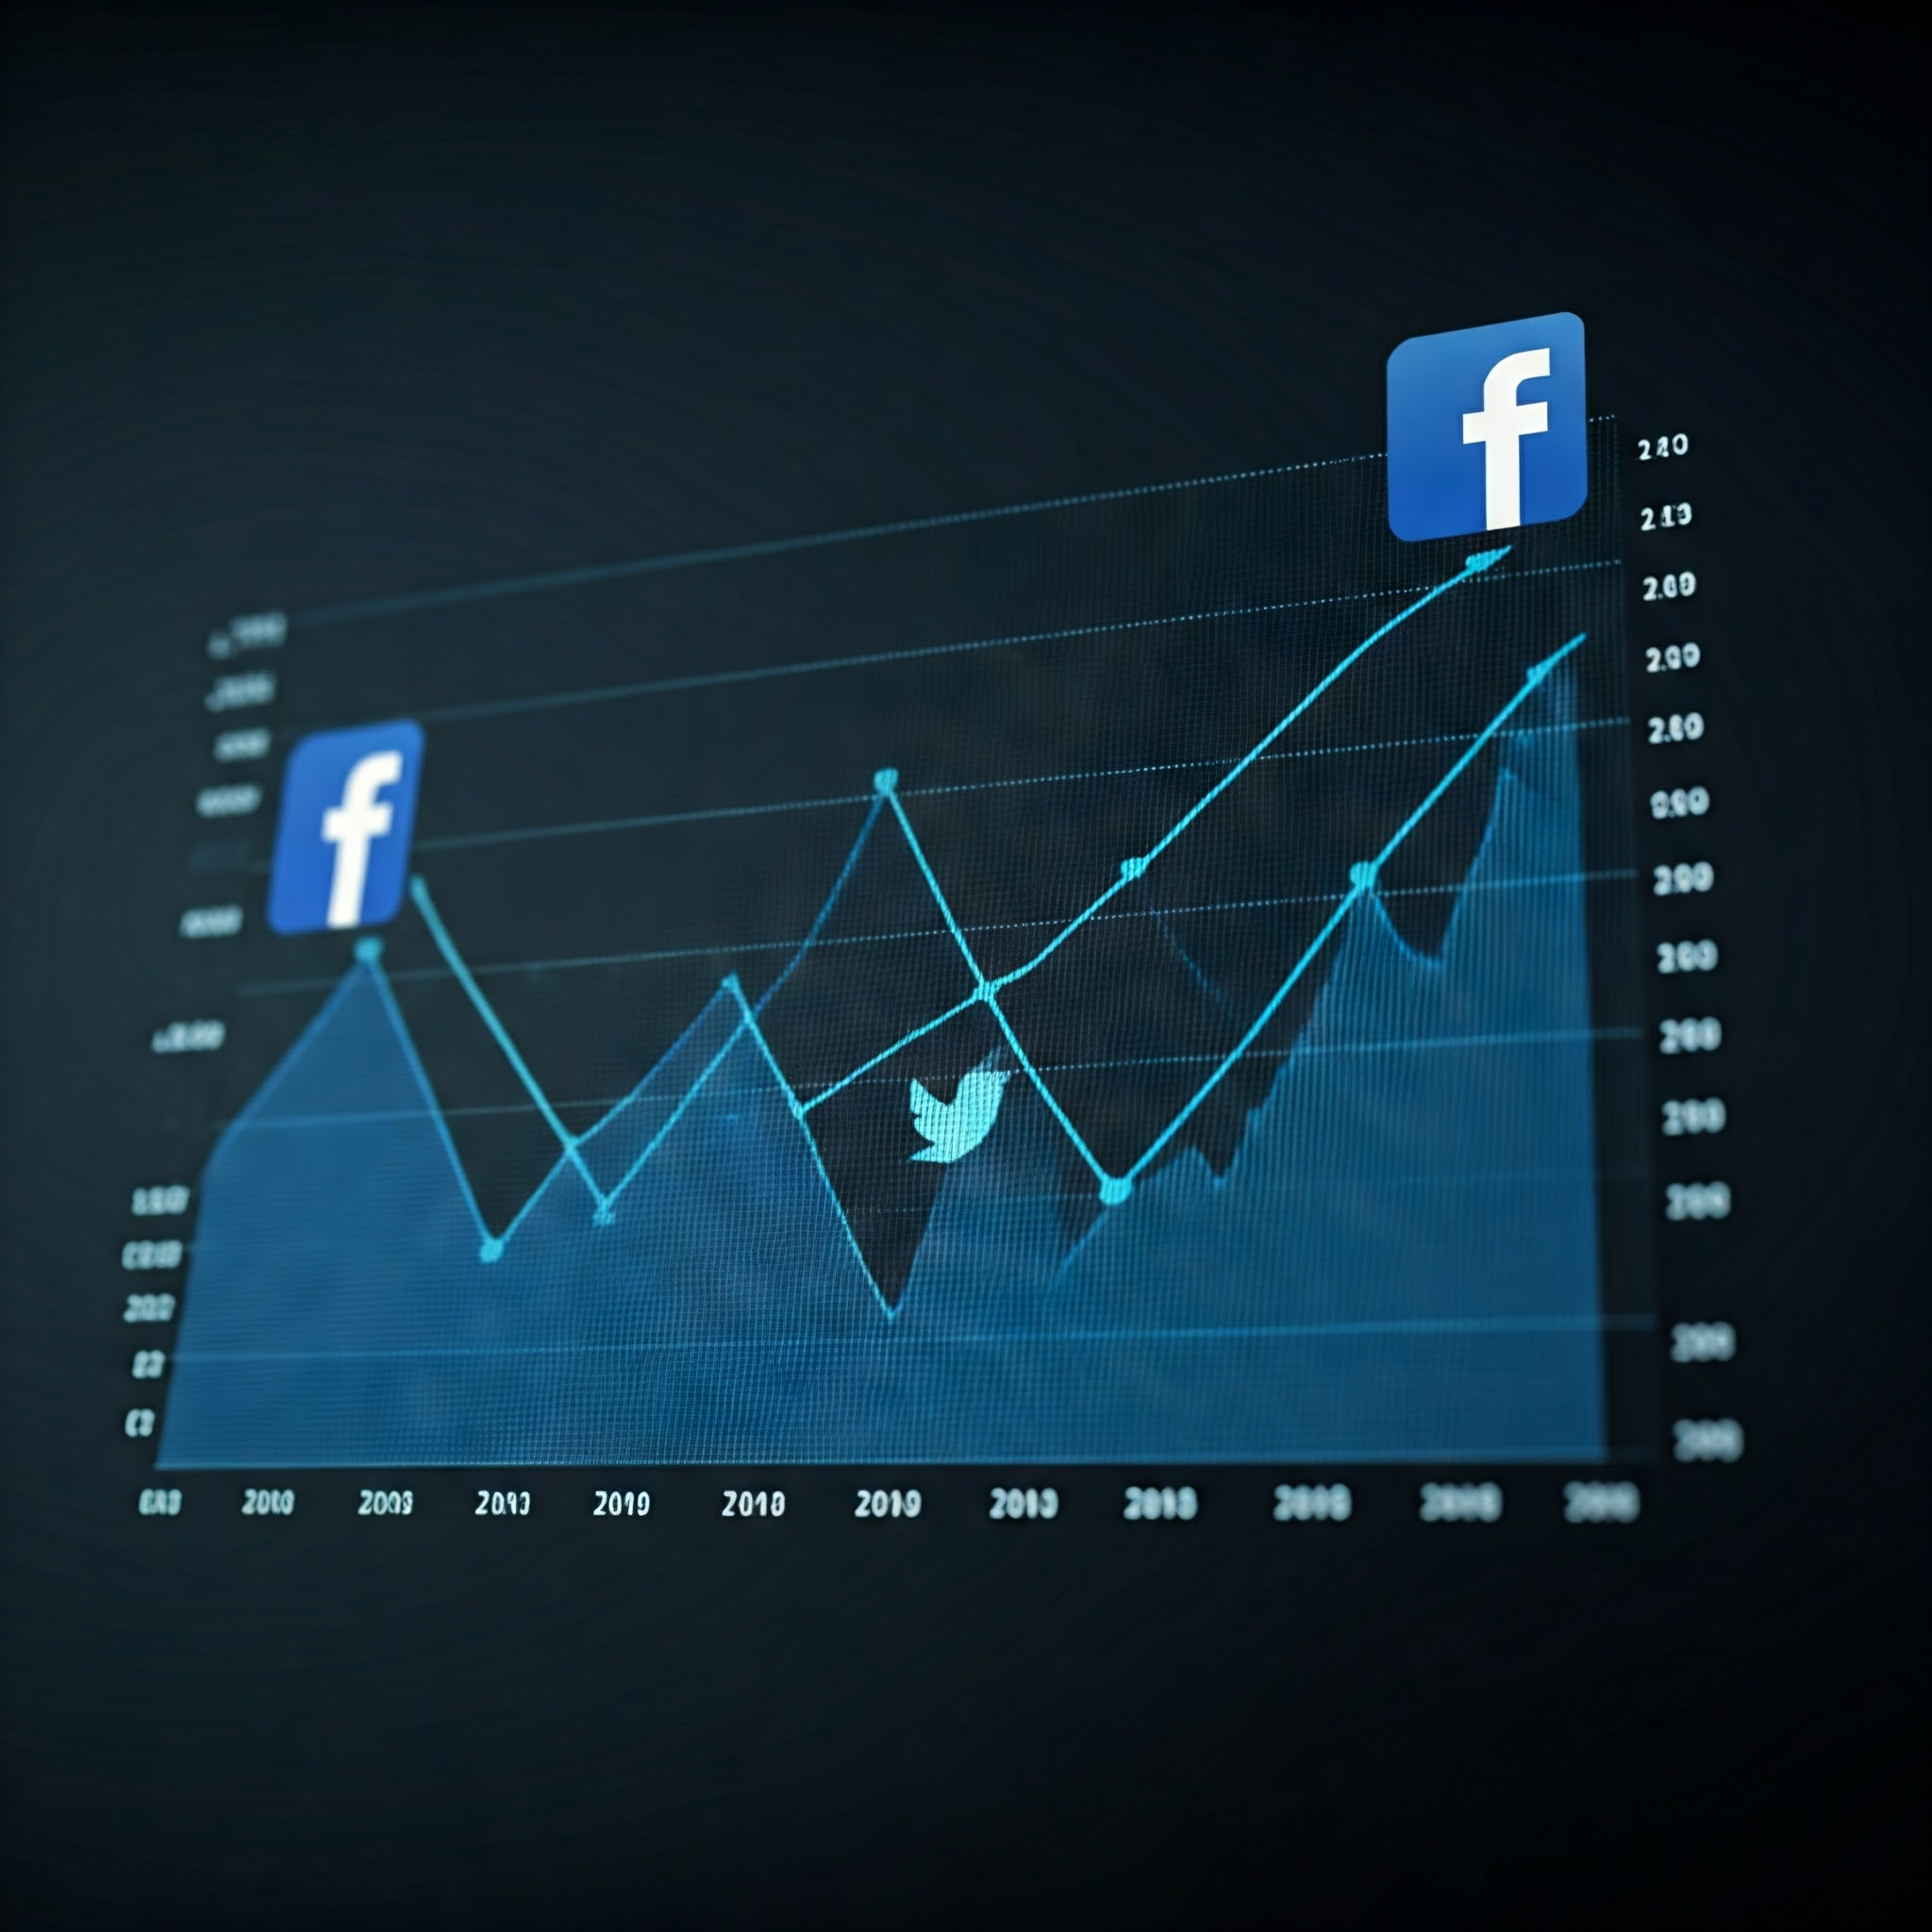
\includegraphics[width=1.35\textwidth, keepaspectratio]{images/introduction_and_motivation_background_slide_image.jpeg}
            \end{center}

            \column{0.75\textwidth}
            \vspace{0.5cm}
            \begin{itemize}
                \item \textbf{Rapid growth of web content and social media:}
                \begin{itemize}
                    \item Over 5.22 billion active social media users globally in 2024\**.
                    \item Platforms include Facebook, Twitter, LinkedIn, Instagram, and others.
                \end{itemize}
            \end{itemize}
        \end{columns}

        \vspace{0.5cm}
        \begin{itemize}
            \item \textbf{Challenges in content management and distribution:}
            \begin{itemize}
                \item Managing the volume of web content is impractical manually.
                \item Ensuring consistency across platforms requires efficient tools.
            \end{itemize}
        \end{itemize}

        \vspace{1.25cm}
        {\tiny \** Source: \url{https://datareportal.com/social-media-users}}
    \end{frame}

    \begin{frame}{Motivation}
        \begin{columns}[T]
            \column{0.27\textwidth}
            \hspace{-0.5cm}
            \vspace{0.2cm}
            \begin{center}
                
\includegraphics[width=1.63\textwidth, keepaspectratio]{images/introduction_and_motivation_motivation_slide_image.png}
            \end{center}

            \column{0.73\textwidth}
            \vspace{0.5cm}
            \begin{itemize}
                \item \textbf{Need for automation:}
                \begin{itemize}
                    \item Optimizes processes, reduces manual effort.
                    \item Ensures consistency and scalability through different platforms.
                \end{itemize}
            \end{itemize}
        \end{columns}

        \vspace{0.5cm}
        \begin{itemize}
            \item \textbf{Gaps in current tools:}
            \begin{itemize}
                \item Many tools focus on single platforms or lack in modularity.
                \item Inadequate metadata handling, particularly for non-standard websites.
                \item Poor adaptability to new platforms or content types.
            \end{itemize}
        \end{itemize}
    \end{frame}


\section{Problem Statement}
    \begin{frame}{Problem Statement}
        \begin{block}{Challenge}
            Managing the continuously growing web content and social media manually is time-consuming, inconsistent, and inefficient.
        \end{block}

        \vspace{0.5cm}

        \begin{alertblock}{Problem}
            Existing tools lack multi-platform integration, modularity, and effective handling of non-standard metadata formats.
        \end{alertblock}

        \vspace{0.5cm}

        \begin{exampleblock}{Solution}
            A scalable, modular solution like SMKIT can ensure consistency and adaptability across diverse content and platforms.
        \end{exampleblock}
    \end{frame}


\section{Objectives}
    \begin{frame}{Objectives}
        \begin{block}{Primary Objective}
            Develop SMKIT to automate and optimize social media and web content management.
        \end{block}

        \begin{itemize}
            \item \textbf{Automating Content Posting:}
                Reduce manual effort and ensure consistent scheduling.
            \vspace{0.3cm}
            \item \textbf{Multi-Platform Support:}
                Smooth integration with platforms like Twitter and Facebook.
            \vspace{0.3cm}
            \item \textbf{Metadata Extraction:}
                \begin{itemize}
                    \item Extract essential metadata like Open Graph tags.
                    \item Handle non-standard metadata efficiently.
                \end{itemize}
            \vspace{0.3cm}
            \item \textbf{Modularity and Scalability:}
                Support feature extensibility and increasing workloads.
        \end{itemize}
    \end{frame}


\section{Overview of SMKIT}
    \begin{frame}{High-Level Architecture}
        \begin{itemize}
            \item Show a diagram of SMKIT’s modular structure.
            \item Highlight generic and specialized modules.
        \end{itemize}
    \end{frame}

    \begin{frame}{Workflow}
        \begin{itemize}
            \item Illustrate the process: input (web pages) → analysis (metadata extraction) → output (social media/web posts).
        \end{itemize}
    \end{frame}

    \begin{frame}{Features}
        \begin{itemize}
            \item Metadata extraction (Open Graph tags, etc.).
            \item Multi-platform content posting (Twitter, Facebook, web).
            \item Customizable templates.
        \end{itemize}
    \end{frame}


\section{Technical Implementation}
    \begin{frame}{Core Components}
        \begin{itemize}
            \item Generic module for Open Graph metadata handling.
            \item Specialized Negapedia module.
        \end{itemize}
    \end{frame}

    \begin{frame}{Metadata Extraction}
        \begin{itemize}
            \item Discuss Open Graph tag analysis and fallback mechanisms.
        \end{itemize}
    \end{frame}

    \begin{frame}{Posting Process}
        \begin{itemize}
            \item Explain integration with social platforms APIs (Facebook, Twitter).
            \item Template usage for consistent identity.
        \end{itemize}
    \end{frame}

    \begin{frame}{Challenges}
        \begin{itemize}
            \item Discuss key technical challenges and solutions (e.g., handling metadata variability, scaling for multiple platforms).
        \end{itemize}
    \end{frame}


\section{Negapedia Module Case Study}
    \begin{frame}{Functionality}
        \begin{itemize}
            \item Summarization, comparison, and ranking modes.
            \item Unique features (conflict, anger levels, etc.).
        \end{itemize}
    \end{frame}

    \begin{frame}{Example Outputs}
        \begin{itemize}
            \item Show a few example posts generated from Negapedia data.
        \end{itemize}
    \end{frame}


\section{Results and Evaluation}
    \begin{frame}{Performance}
        \begin{itemize}
            \item Highlight results from testing (e.g., metadata extraction accuracy, processing time).
        \end{itemize}
    \end{frame}

    \begin{frame}{Effectiveness}
        \begin{itemize}
            \item Metrics like engagement improvements or user feedback.
        \end{itemize}
    \end{frame}

    \begin{frame}{Comparison with Existing Tools}
        \begin{itemize}
            \item Briefly discuss how SMKIT addresses gaps better than existing tools.
        \end{itemize}
    \end{frame}


\section{Contributions and Future Work}
    \begin{frame}{Contributions}
        \begin{itemize}
            \item Summarize key contributions of your thesis (e.g., modular framework, specialized Negapedia module, open-source tool).
        \end{itemize}
    \end{frame}

    \begin{frame}{Future Work}
        \begin{itemize}
            \item Discuss potential extensions (e.g., more modules, support for additional platforms).
        \end{itemize}
    \end{frame}


\section{Conclusion}
    \begin{frame}{Conclusion}
        \begin{itemize}
            \item Discuss potential extensions Recap the problem, solution (SMKIT), and key results.
            \item Closing statement on the significance of your work.
        \end{itemize}
    \end{frame}


\begin{emptyframe}
     \textbf{ \textit{Thank you!} }
\end{emptyframe}

\appendix
    
\end{document}